\chapter{Дүрстэй танилцах}
\section{Зурагны хэмжээ боловсруулах}
Энэ үйл явцын эхний алхам нь авч үзэж буй зураг бүр ижил хэмжээтэй байхыг шалгах явдал юм. Энэ нь өөр өөр зургуудыг харьцуулах боломжийг олгох тул, маш чухал юм. Хэмжээний аливаа ялгаа нь алдаатай үр дүн эсвэл буруу үр дүнд хүргэх, эсвэл бүр дундаж утгыг тооцолох боломжгүй байдалд хүргэнэ. Тиймээс бид дараагийн алхам руу шилжихээсээ өмнө өгөгдлийн  дэх зураг бүрийн хэмжээг стандарт хэмжээ болгон өөрчлөх хэрэгтэй.

\section{Дундаж зураг тооцоолох}
Бүх зургийн хэмжээг стандартчилсны дараа бид дундаж зургийг тооцоолж болно. Бүх зураг дээрх харгалзах пикселийн байрлал бүрийн дундаж утгыг тооцоолох замаар дундаж зургийг олж авна. Энэ процессын үр дүнд өгөгдлийн багц дахь бүх зургийн "дундаж"-ыг илэрхийлэх нэг зураг гарч, бүх зургийн нийтлэг шинж чанаруудыг үр дүнтэйгээр гарган авах боломжтой.

\begin{lstlisting}[language=Python, caption=Дундаж зураг тооцоолох код, frame=single]
import os
import cv2

current_directory = os.getcwd()

items = os.listdir(current_directory + "/images")
jpgs = [item for item in items if "jpg" in item]
jpg_len = len(jpgs)
avg_image = 0

gray_img_list = []

for item in items:
    if "jpg" in item:
        try:
            image = cv2.imread(current_directory + "/images/" + item)
            print(item, "is read")
            resized_image = cv2.resize(image, [500, 500])
            gray_image = cv2.cvtColor(resized_image, cv2.COLOR_RGB2GRAY)
            gray_img_list.append(gray_image)
            avg_image += gray_image / jpg_len
        except Exception as e:
            print(e)

for gray_img, jpg in zip(gray_img_list, jpgs):
    result = avg_image - gray_img
    if not os.path.exists(current_directory + "/result"):
        os.makedirs(current_directory + "/result")
    cv2.imwrite(
        current_directory + "/result/" + str(jpg) + "_gray_avg" + ".jpg",
        result,
    )
	\end{lstlisting}
	
\section{Зургийн ялгааг олох}
Дараагийн шат нь өгөгдлийн багц дахь зураг бүрээс дундаж зургийг хасах явдал юм. Энэ алхамын зорилго нь зураг тус бүр болон дундаж зураг хоорондын ялгааг тодруулах явдал юм. Үүний үр дүнд тус бүр нь дунджаас ялгарах зургийн өвөрмөц онцлогийг илэрхийлэх "ялгаатай зураг"-ийн багц үүснэ. Ялгаатай зургуудыг дараа нь сонирхолтой байж болох өвөрмөц хэв эсвэл гажигийг тодорхойлоход ашиглаж болно.

\section{Нэмэлт мэдээлэл}

Компьютерт зургийг массив байдлаар дүрсэлдэг энэ нь RGB буюу Red, Green, Blue гэсэн гурван өнгийг илэрхийлэх ба зарим тохиолдолд Alpha channel нэмэгдэх ба энэ нь массивын уртыг нэгээр нэмэх бөгөөд өнгөний тодролийг илгтэнэ.

Зургийг матрицаар илэрхийлж болж байгаа учир адилхан хэмжээтэй зурагнууд дээр математик үйлдлүүд хийх боломжтой болох юм. Тухайлвал олон зурагны дунджийг олж болох ба, энэ нь матриц дээр математик үйлдлүүд цаанаа хийгдэх хэдий ч хэрэглэгчид харагдахдаа зурагнуудыг хооронд нь нийлүүлсэн мэт мэдрэмжийг төрүүлнэ.

\section{Кодны тайлбар}
Python хэл ашигласан бөгөөд `OS` санг ашиглан фолдер дотор байгаа бүх зургийн замыг авч чадна, дараагаар нь зураг бүрийг тус тусад нь уншиж тэр бүрдээ дундаж зургийг өөрчилнө.



\begin{lstlisting}[language=Python, caption=Дундаж зураг тооцоолох код, frame=single]
items = os.listdir(current_directory + "/images")
\end{lstlisting}

\begin{lstlisting}[language=Python, caption=Дундаж зураг тооцоолох код, frame=single]
	for item in items:
    if "jpg" in item:
        try:
            image = cv2.imread(current_directory + "/images/" + item)
            print(item, "is read")
            resized_image = cv2.resize(image, [500, 500])
            gray_image = cv2.cvtColor(resized_image, cv2.COLOR_RGB2GRAY)
            gray_img_list.append(gray_image)
            avg_image += gray_image / jpg_len
        except Exception as e:
            print(e)
\end{lstlisting}

Зурагны ялгааг олохдоо шууд `-` эсвэл `+` тэмдэг ашиглан математик үйлдэл хийж болно.

\section{Дүгнэлт}

Энэ тайланд авч үзсэн зургийн хэмжээсийг хэвийн болгох, дундаж зургийн тооцоолол, ялгааг тооцоолох арга нь хэв танилтын салбарт хүчирхэг хэрэгсэл юм. Энэ нь өгөгдлийн багц дахь нийтлэг болон өвөрмөц шинж чанаруудыг тодорхойлох боломжийг олгодог бөгөөд ингэснээр өгөгдөлд байгаа хэв маягийн талаар цогц ойлголтыг өгдөг. Энэ нь нүүр царай таних, гажиг илрүүлэх гэх мэт төрөл бүрийн хэрэглээтэй билээ.
\appendix
\addcontentsline{toc}{part}{ХАВСРАЛТ}

% Хавсралтын нэр. Хавсралт гэдэг үг агуулахгүй
\chapter{Жишээ зурагнууд}
\begin{figure}
	\centering
	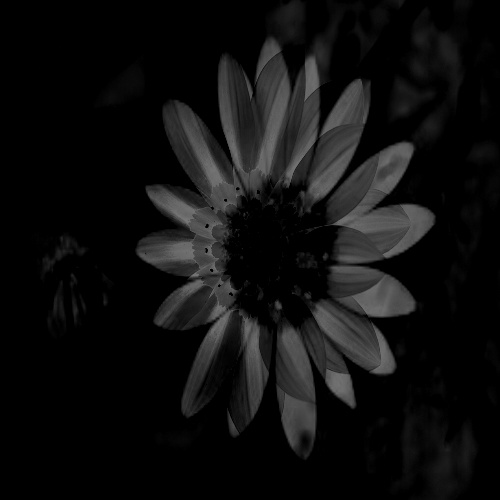
\includegraphics[scale=0.8]{src/img/pic1.png}
	\caption{Жишээ-1}
\end{figure}
\begin{figure}
	\centering
	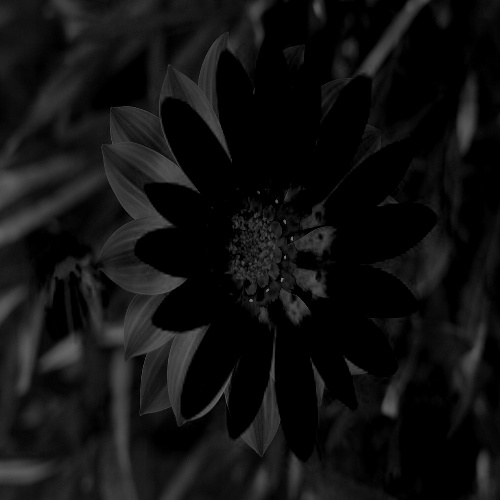
\includegraphics[scale=0.8]{src/img/pic2.png}
	\caption{Жишээ-2}
\end{figure}


% Хавсралтын нэр. Хавсралт гэдэг үг агуулахгүй